\begin{tabular}{lrrrrrrrrrrrr}
\toprule
BENCHMARK                          & b.sort            &  h.sort           & b.srch            & fft               & xxtea             & md5               & rc5               & coremk            & \makebox[0.2mm]{}   & average           \\
\hline
\multicolumn{10}{l}{EXECUTED JVM INSTRUCTIONS (\%)} \\
% Take this from results_0BASE_R___P__C0_A1_S0_G1 (16-bit array index enabled), otherwise we will get a lot of S2I conversions since the code uses shorts.
\xxt Load/Store                    &              79.8 &              72.1 &              58.8 &              57.8 &              50.9 &              43.7 &              41.1 &            55.5   &     &              57.5 \\
\xxt Constant load                 &               0.2 &               8.1 &               9.8 &              10.8 &              12.5 &              19.1 &              17.6 &            10.1   &     &              11.0 \\
\xxt Processing                    &               8.0 &               7.8 &              13.1 &              22.8 &              32.4 &              28.9 &              36.6 &            14.0   &     &              20.5 \\
  \xxxt   math                     & \xt           8.0 & \xt           5.6 & \xt           9.2 & \xt          12.0 & \xt          10.1 & \xt          12.5 & \xt          10.7 & \xt         8.3   &     & \xt           9.6 \\
  \xxxt   bit shift                & \xt           0.0 & \xt           2.3 & \xt           3.9 & \xt           7.5 & \xt           8.1 & \xt           5.4 & \xt           8.0 & \xt         2.2   &     & \xt           4.7 \\
  \xxxt   bit logic                & \xt           0.0 & \xt           0.0 & \xt           0.0 & \xt           3.2 & \xt          14.2 & \xt          11.0 & \xt          17.9 & \xt         3.6   &     & \xt           6.2 \\
\xxt Branches                      &              12.0 &              11.0 &              17.6 &               4.1 &               4.0 &               5.8 &               2.3 &            16.0   &     &               9.1 \\
\xxt Invoke                        &               0.0 &               0.5 &               0.0 &               0.0 &               0.0 &               0.0 &               0.0 &             0.4   &     &               0.1 \\
\xxt Others                        &               0.0 &               0.5 &               0.7 &               4.5 &               0.2 &               2.5 &               2.4 &             4.0   &     &               1.9 \\
% Take this from results_0BASE_R___P__C0_A1_S0_G1 as well.
\multicolumn{10}{l}{STACK} \\
\xxt Max. stack (bytes)            &                 8 &                 8 &                 8 &                 8 &                24 &                20 &                14 &              18   &     &              13.5 \\
\xxt Avg. stack (bytes)            &               2.6 &               2.9 &               2.8 &               3.0 &              11.8 &               6.3 &               6.8 &             3.2   &     &               4.9 \\
\hline
\multicolumn{10}{l}{PERFORMANCE OVERHEAD BEFORE OPTIMISATIONS (\%)} \\
% Take this from main-performance-graph.xlsx 
\xxt Total                         &             496.7 &             351.4 &             430.8 &             522.6 &             251.5 &             226.5 &             123.4 &           359.0   &     &             345.2 \\
  \xxxt push/pop                   & \xt         183.5 & \xt         139.4 & \xt         192.5 & \xt         220.2 & \xt         168.0 & \xt         105.9 & \xt          61.3 & \xt       128.2   &     & \xt         149.9 \\
  \xxxt load/store                 & \xt         200.1 & \xt         144.3 & \xt         180.9 & \xt         132.7 & \xt          42.5 & \xt          43.9 & \xt          28.5 & \xt        91.9   &     & \xt         108.1 \\
  \xxxt mov(w)                     & \xt          10.4 & \xt           2.9 & \xt          -1.2 & \xt           6.2 & \xt           2.4 & \xt           1.7 & \xt          -1.7 & \xt         4.0   &     & \xt           3.1 \\
  \xxxt other                      & \xt         102.7 & \xt          64.8 & \xt          58.7 & \xt         163.5 & \xt          38.6 & \xt          75.0 & \xt          35.3 & \xt       134.9   &     & \xt          84.2 \\
\multicolumn{10}{l}{PERFORMANCE OVERHEAD REDUCTION PER OPTIMISATION (\%)} \\
\xxt Impr. peephole                &            -162.8 &            -118.8 &            -116.3 &             -99.9 &             -61.8 &             -51.7 &             -23.2 &           -61.0   &     &             -86.9 \\
\xxt Stack caching                 &             -22.9 &             -29.5 &             -76.8 &            -129.8 &             -97.3 &             -54.3 &             -38.6 &           -40.0   &     &             -61.1 \\
\xxt Pop. val. caching             &            -116.6 &             -73.3 &             -29.8 &             -52.4 &              -6.9 &             -12.9 &              -8.8 &           -26.0   &     &             -40.9 \\
\xxt Mark loops                    &             -62.3 &             -28.8 &             -84.4 &             -40.2 &              +5.1 &             -10.9 &              -8.1 &           -40.4   &     &             -33.7 \\
\xxt Const shift                   &               0.0 &              -9.2 &             -22.4 &             -80.4 &             -18.5 &             -43.8 &             -20.2 &           -10.2   &     &             -25.6 \\
\xxt 16-bit array index            &             -37.5 &             -25.3 &             -36.5 &             -22.4 &             -13.8 &              -5.5 &              -4.1 &           -39.3   &     &             -23.1 \\
\xxt SIMUL                         &               0.0 &               0.0 &               0.0 &               0.0 &               0.0 &               0.0 &               0.0 &           -36.7   &     &              -4.6 \\
\multicolumn{10}{l}{PERFORMANCE OVERHEAD AFTER OPTIMISATIONS (\%)} \\
\xxt Total                         &              94.6 &              66.5 &              64.6 &              97.5 &              58.3 &              47.4 &              20.4 &           105.4   &     &             69.3 \\
  \xxxt push/pop                   & \xt           0.0 & \xt          -7.0 & \xt           0.0 & \xt           0.0 & \xt          37.4 & \xt           0.1 & \xt           2.9 & \xt         5.1   &     & \xt          4.8 \\
  \xxxt load/store                 & \xt           9.0 & \xt          33.2 & \xt          28.2 & \xt          22.5 & \xt          -2.3 & \xt          20.3 & \xt           4.3 & \xt        17.6   &     & \xt         16.6 \\
  \xxxt mov(w)                     & \xt          10.4 & \xt           3.9 & \xt          10.8 & \xt           4.6 & \xt           5.6 & \xt           2.2 & \xt           0.5 & \xt        10.0   &     & \xt          6.0 \\
  \xxxt other                      & \xt          75.3 & \xt          36.4 & \xt          25.6 & \xt          70.4 & \xt          17.6 & \xt          24.8 & \xt          12.7 & \xt        72.7   &     & \xt         41.9 \\
\bottomrule
\end{tabular}   



\section{AOT translation: performance}
\label{sec-evaluation-aot-translation-performance}

Next we will look at the effect of our optimisations to the baseline AOT translation approach, for all our benchmarks.

The trace data produced by Avrora gives us a detailed view into the run-time performance and the different types of overhead. We count the number of bytes and cycles spent on each native instruction for both the native C and our AOT compiled version, and group them into 4 categories that roughly match the types of AOT translation overhead discussed in Section \ref{sec-overhead-aot-translation}:
\begin{itemize}
	\item \mycode{PUSH},\mycode{POP}: Matches the type 1 push/pop overhead since native code uses almost no push/pop instructions.
	\item \mycode{LD},\mycode{LDD},\mycode{ST},\mycode{STD}: Matches the type 2 load/store overhead and directly shows the amount of memory traffic.
	\item \mycode{MOV},\mycode{MOVW}: For moves the picture is less clear since the AOT compiler emits them for various reasons. Before we introduce stack caching, it emits moves to replace push/pop pairs, and after the mark loops to save a pinned value when it is popped destructively.
	\item others: the total overhead, minus the previous three categories. This roughly matches the type 3 overhead.
\end{itemize}

We define the overhead from each category as the number of bytes or cycles spent in the AOT version, minus the number spent by the native version for that category, and again normalise this to the \emph{total} number of bytes or cycles spent in the native C version. The detailed results for each benchmark and type of overhead are shown in tables \ref{tbl-performance-per-benchmark} and \ref{tbl-codesize-per-benchmark}. In addition, Table \ref{tbl-performance-per-benchmark} also lists the time spent in the VM on method calls.

In Figure \ref{fig-performance-per-opcode-category} we see how our optimisations combine to reduce performance overhead. We take the average of all benchmarks, and show both the total overhead, and the overhead for each instruction category. Figure \ref{fig-performance-per-benchmark} shows the total overhead for each individual benchmark. We start with the original AOT approach with only the simple peephole optimiser, and then incrementally add each of our optimisations. The lightweight method call optimisation is already included in these results. We will examine its effect separately in Section \ref{sec-evaluation-method-invocation}.

\begin{figure}
\centering
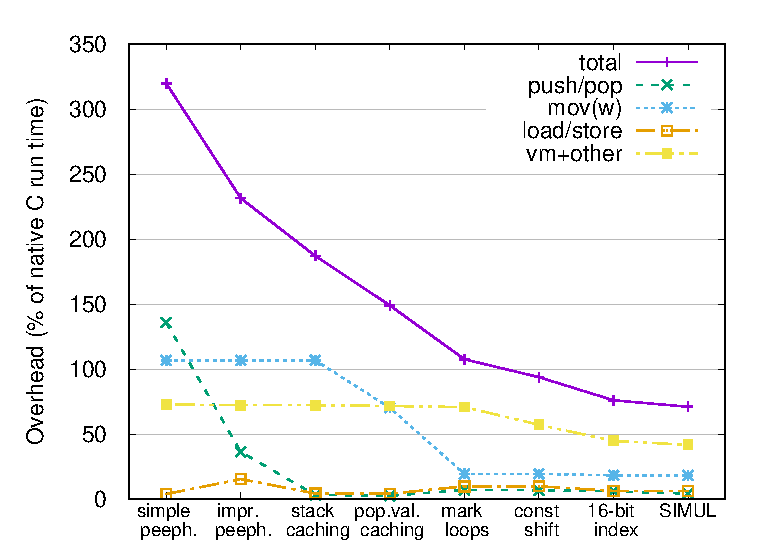
\includegraphics[width=\mygraphsize]{performance-per-opcode-category.eps}
\caption{Performance overhead per category}
\label{fig-performance-per-opcode-category}
\end{figure}

\begin{figure}
\centering
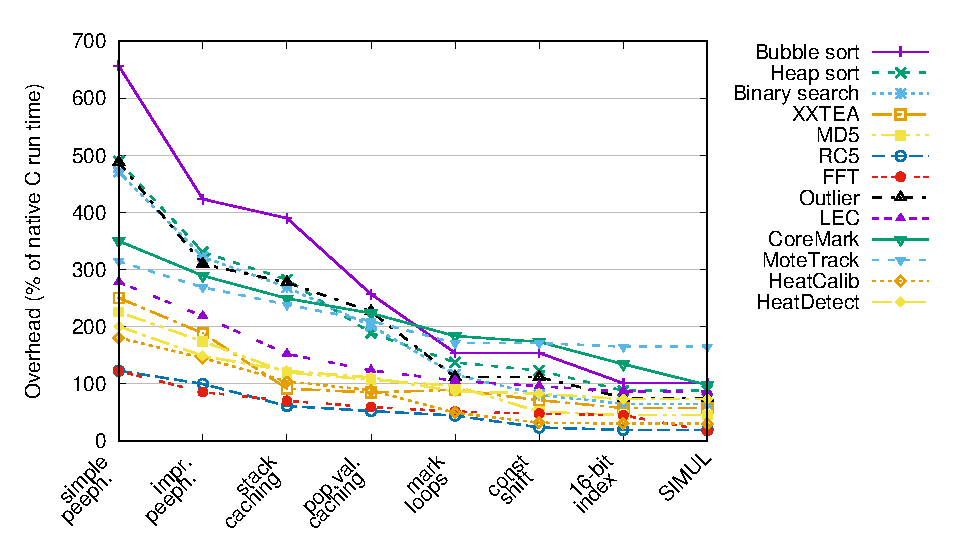
\includegraphics[width=\mygraphsize]{performance-per-benchmark.eps}
\caption{Performance overhead per benchmark}
\label{fig-performance-per-benchmark}
\end{figure}

Using the simple optimiser, the types 1, 2 and 3 overhead are all significant, at 136\%,  107\%, and 70\% respectively. The basic approach does not have many reasons to emit a move, so we see that in some cases the AOT version actually spends fewer cycles on move instructions than the C version, resulting in small negative values.  When we improve the peephole optimiser to include non-consecutive push/pop pairs, push/pop overhead drops by 99.4\% (of native C performance), but if the push and pop target different registers, they are replaced by a move instruction, and we see an increase of 11.5\% in move overhead. For a 16-bit value this takes 1 cycle (for a MOVW instruction), instead of 8 cycles for two pushes and two pops. The increase in moves shows most of the extra cases that are handled by the improved optimiser are replaced by a move instead of eliminated, since the 11.5\% extra move overhead matches a 92\% reduction in push/pop overhead.

Next we introduce stack caching to utilise all available registers and eliminate most of the push/pop instructions that cannot be handled by the improved optimiser. As a result the push/pop overhead drops to nearly 0, and so does the move overhead since most of the moves introduced by the peephole optimiser, are also unnecessary when using stack caching.

Having eliminated the type 1 overhead almost completely, we now add popped value caching to remove a large number of the unnecessary load instructions. This reduces the memory traffic significantly, as is clear from the reduced load/store overhead, while the other types remain stable. Adding the mark loops optimisation further reduces loads, and this time also stores, by pinning common variables to a register. But it uses slightly more move instructions, and the fact that we have fewer registers available for stack caching means we have to spill stack values to memory more often. While we save 50.8\% on loads and stores, the push/pop and move overhead increase by 4.5\% and 5.7\% respectively.

Most of the push/pop and load/store overhead has now been eliminated and the type 3 overhead, unaffected by these optimisations, has become the most significant source of overhead. This type has many different causes, but we can eliminate part of it with our three instruction set optimisations. These optimisations, especially the 16-bit array index, also reduce register pressure, so we also see slight decreases in the other overhead types, although this is minimal in comparison. The CoreMark and FFT benchmarks are the only ones to do 16-bit to 32-bit multiplication, so the average performance improvement for \mycode{SIMUL} is small, but Table \ref{tbl-performance-per-benchmark} shows it is significant for these two benchmarks.

Combined, these optimisations reduce performance overhead from 320\% to 71\% of native C performance.
